\problemname{Developer}
You are in charge of developing new properties in the suburbs of Toruń.
You have already decided that there will be one main street and $n$ properties
numbered from $1$ to $n$ along the street. The area is somewhat hilly,
and the elevation of the $i$-th property is $a_{i}$ centimetres.

It turns out that no one wants to
buy a property that is on a \emph{slope}.
Formally, for elevations $a_1, a_2, \dots, a_n$, a slope is
a contiguous subsequence $a_{i-1}, a_i, \dots, a_j, a_{j+1}$ with $2 \leq i\leq j\leq n-1$ such that
either (i) $a_{i-1} < a_{i}=a_{i+1}=\ldots=a_{j}  < a_{j+1}$, or (ii) $a_{i-1} > a_{i}=a_{i+1}=\ldots=a_{j} > a_{j+1}$.
Intuitively, a slope is a contiguous range of properties at positions $i-1, i, i+1, \ldots, j, j+1$,
where the elevations of all properties at positions $i,i+1,\ldots,j$ are equal to some $h$, and $h$ is strictly between
$a_{i-1}$ and $a_{j+1}$. 

You are able to increase or decrease the
elevation of any property by any integer, but of course you want to minimise the overall effort.
Your task is to determine the minimal total change in elevation such that there are no slopes at all.
That is, you want to find elevations $b_1, b_2, \dots, b_n$ without slopes
such that $|a_1 - b_1| + |a_2 - b_2| + \dots + |a_n - b_n|$ is as small as possible.
The elevations $b_i$ must be integers (in particular, they don't have to be positive),
and there are no other constraints on $b_i$.
 
\section*{Input}
The first line contains an integer $n$ ($1\leq n\leq 2 \cdot 10^{5}$) denoting the number of properties
along the street.

The second line contains $n$ integers $a_{1}, a_{2}, \ldots, a_{n}$ ($0\leq a_{i} \leq 10^{9}$),
where the $i$-th integer $a_{i}$ is the initial elevation of the $i$-th property.

\section*{Output}
You should output the minimal total change in elevation to ensure that there are no slopes.

\section*{Scoring}
\begin{center}
\begin{tabular}{|c|p{13cm}|c|}
\hline
\textbf{Subtask} & \textbf{Constraints} & \textbf{Points} \\ \hline
1 & $n \leq 5$ and $a_{i} \leq 10$ & 4 \\\hline
2 & $n \leq 2000$ & 13 \\\hline
3 & $a_{i}\leq 10$ & 8 \\\hline
4 & $a_{i} < a_{i+1}$ & 19 \\\hline
5 & $n \leq 2\cdot10^4$ & 29 \\\hline
6 & No additional constraints. & 27 \\\hline
\end{tabular}
\end{center}

\section*{Explanation of sample 1}
The first sample is illustrated below.
The dashed lines represent the changed elevations without slopes $b_i$ of their corresponding properties.

\begin{center}
\begin{figure}[h!]
    \centering
    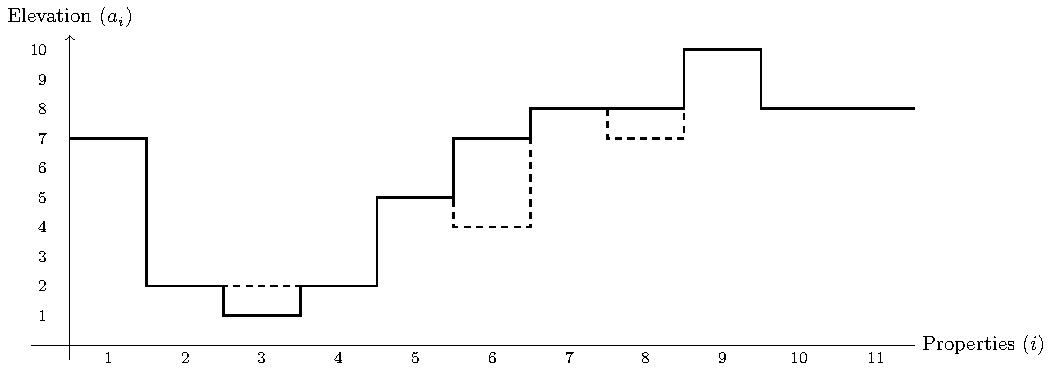
\includegraphics[width=1\textwidth]{heights.pdf}
\end{figure}
\end{center}
